% Autor: Matthias Götz

\section{Karte}

\subsection{Standardkarte}

Im Bereich "Karte" ist eine Google-Map eingebunden, die den Standort der Hochschule Regensburg anzeigt, siehe Graphik \ref{fig:Karte}.

\begin{figure}[!htbp]
 \centering
 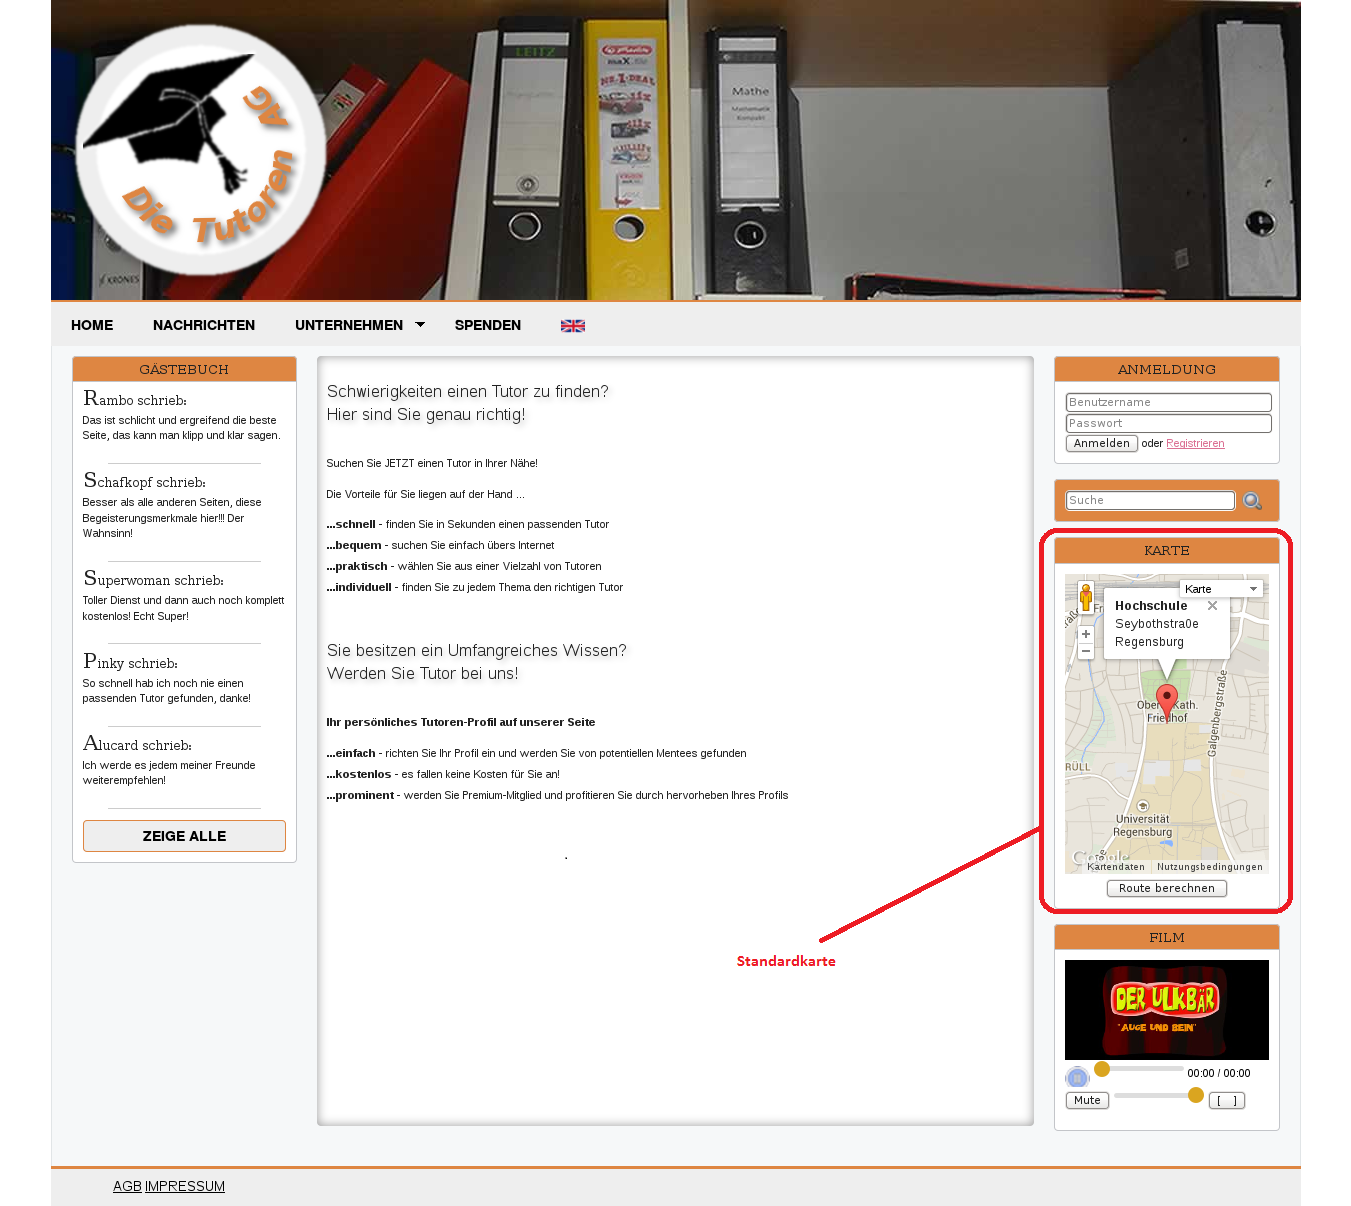
\includegraphics[width=1\textwidth]{../Screenshots/Karte}
 \caption{Standardkarte}
 \label{fig:Karte}
\end{figure}

\newpage

\subsection{Berechnete Route}

Durch Klicken des Buttons "Route berechnen" wird die Route vom aktuellen Standort in die Siemensstraße 12 (Regensburg) berechnet und angezeigt, siehe Graphik \ref{fig:Karte_route}.

\begin{figure}[!htbp]
 \centering
 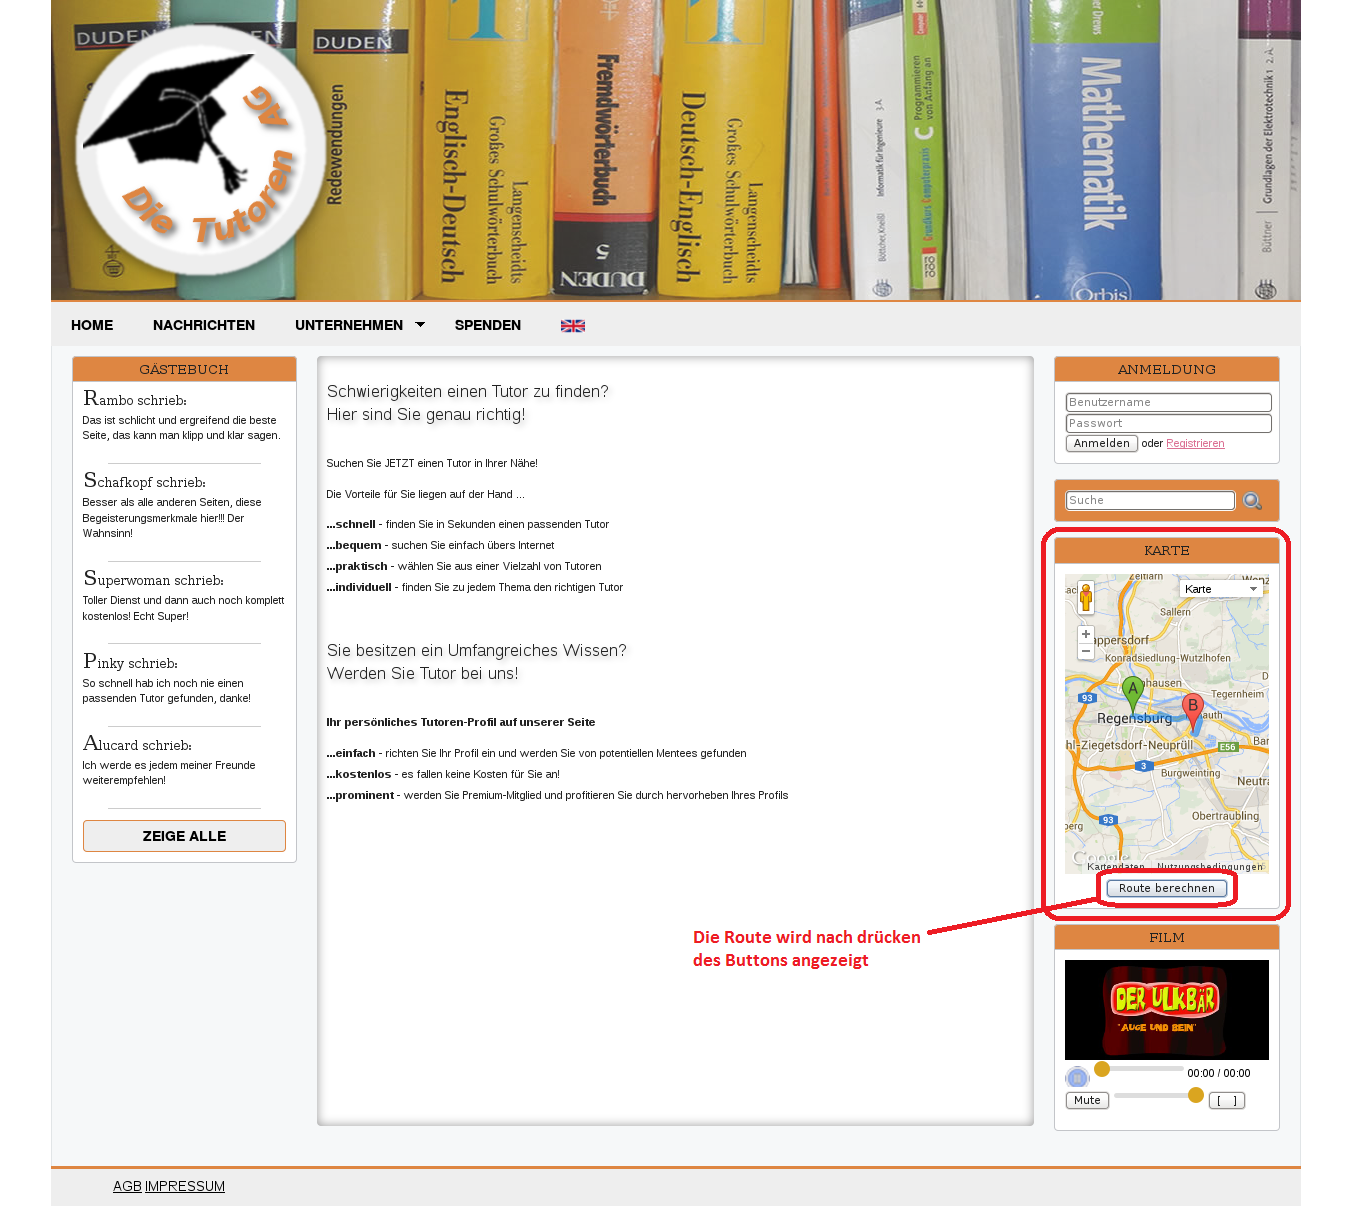
\includegraphics[width=1\textwidth]{../Screenshots/Karte_route}
 \caption{Karte mit berechneter Route}
 \label{fig:Karte_route}
\end{figure}
